%!TEX root = ../../dokumentation.tex

\chapter{Theoretische Grundlagen}

Das folgende Kapitel dient einem besseren Verständnis von Problemstellung und Zielsetzung und bietet einen Überblick über den 
ktuellen Stand der Forschung und aktuelle Entwicklungen im Themenbereich der Cloud Migration.

\section{Cloud Computing}

Im folgenden Unterkapitel werden die Grundlagen und eine Definition des Cloud Computing erarbeitet. Hierbei werden die Grundlegenden Konzepte, Bereitstellungsmodelle und Abstraktionsebenen des Cloud Computing erläutert.

\subsection{Was ist Cloud Computing}

Nach dem \ac{NIST}, auf dessen Definition sich in jüngerer Literatur häufig bezogen wird \cite[Vgl.][S. 4f]{Reinheimer2018}, ist Cloud Computing ein Modell der Zurverfügungstellung von Computing Ressourcen (z.B. Netzwerke, Server, Speicher, Anwendungen und Services),die über das Netzwerk erreichbar sind und mit geringem Managementaufwand schnell freigegeben und bereitgestellt werden können \cite[Vgl.][S. 2]{Mell2011}\cite[Vgl.][S. 5]{Reinheimer2018}.

\begin{wrapfigure}{r}{0.45\textwidth}
\centering
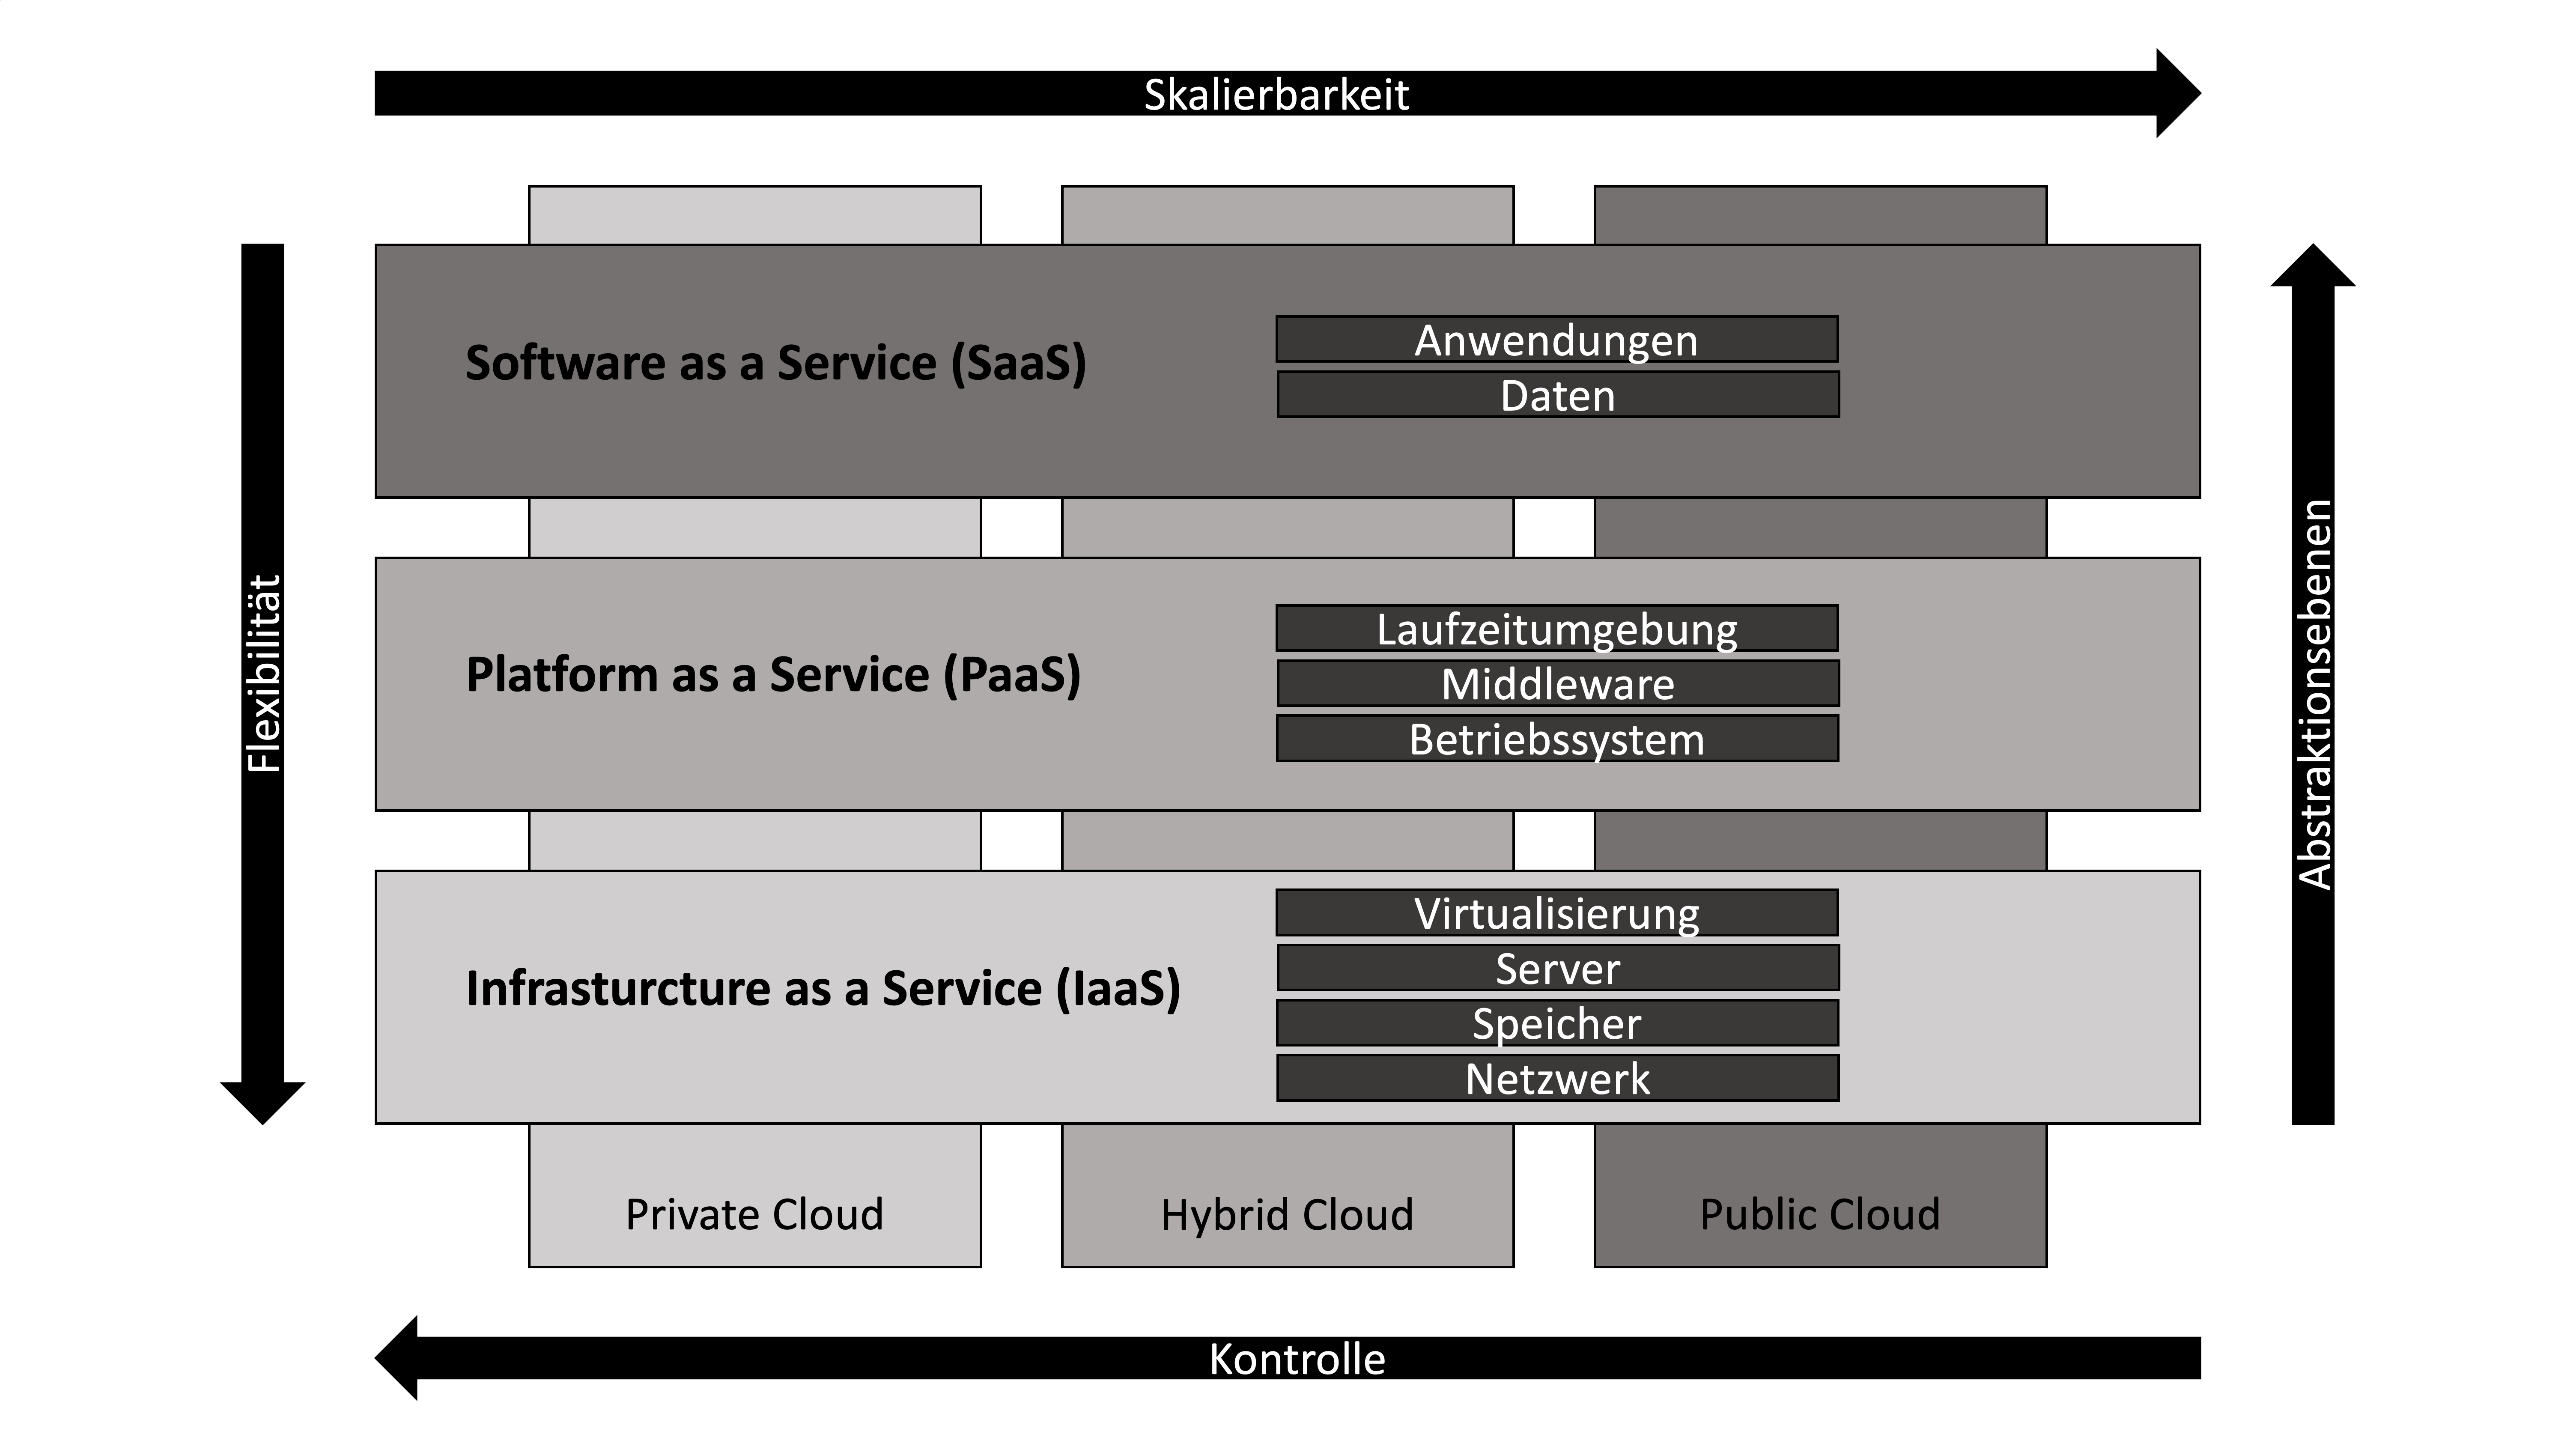
\includegraphics[height=0.3\textwidth]{xaas.png}
\caption{Eine Übersicht der Cloud Service Modelle \cite[Eigene Darstellung nach][S. 33]{Maenhaut2016}\cite[Ergänzt durch][]{Toroman2018}}
\label{fig:XaaS}
\end{wrapfigure}

Nach Hentschel und Leyh (2018), Zhao (2014), Maenhaut (2016) und Surianarayanan (2019) kann man Cloud Services grundsätzlich in drei Abstraktionsebenen einteilen. Diese sind \textbf{\ac{SaaS}}, \textbf{\ac{PaaS}} und \textbf{\ac{IaaS}}, welche auch zu \ac{XaaS} zusammengefasst werden \cite[Vgl.][S. 9]{Reinheimer2018}\cite[Vgl.][S. 143f]{Zhao2014}\cite[Vgl.][S. 32ff]{Maenhaut2016} und \cite[Vgl.][S. 226ff]{Surianarayanan2019}.

Die in Abbildung \ref{fig:XaaS} dargestellte unterste der drei genannten Abstraktionsschichten ist \ac{IaaS}, welche die Basisinfrastruktur, wie zum Beispiel Netzwerk, Server oder Speicher, bereitstellt.

Diese Infrastruktur kann sowohl physisch als auch virtuell zur Verfügung gestellt werden \cite[Vgl.][S. 9f]{Reinheimer2018}. Die darüberliegend dargestellte Schicht ist \ac{PaaS}, welche zu der Infrastrukturebene zusätzlich noch eine Basis zur Anwendungsentwicklung bietet, indem zum Beispiel bereits ein Betriebssystem und Middleware und eine Laufzeitumgebung bereitgestellt werden \cite[Vgl.][S. 10]{Reinheimer2018}. Die oberste Abstraktionsebene ist \ac{SaaS}, welche standardisierte Anwendungen zur Verfügung stellt und sich somit direkt an den Endnutzer richtet und ohne Verwaltung der zugrundeliegenden Ressourcen genutzt werden kann. Diese wird vom Provider übernommen.
\cite[Vgl.][S. 11]{Reinheimer2018}.

Generell wird die Cloud darüber hinaus in drei Organisationsdimensionen eingeteilt \cite[Vgl. auch im Folgenden][S. 7ff]{Reinheimer2018}:
\begin{itemize}
\item \textbf{Private Cloud:} Die Private Cloud bietet die exklusive Nutzung durch eine Organisation der darunterliegenden Infrastruktur. Die IT-Infrastruktur einer Private Cloud kann entweder im Unternehmenseigenen Rechenzentrum untergebracht oder auch von Dienstleistern bereitgestellt werden.
\item \textbf{Public Cloud:} In der Public Cloud ist die Infrastruktur für mehr Anwender zugänglich und muss geteilt werden. Dafür muss als Anwender oft auch nur für die tatsächlich genutzte Leistung gezahlt werden. Da die Infrastruktur jedoch gleichzeitig von vielen genutzt wird, ist zum Beispiel der Betrieb von sicherheitskritischen Anwendungen schwierig.
\item \textbf{Hybrid Cloud:} Die Hybrid Cloud bildet eine kombinierte Anwendung aus der Public Cloud und der Private Cloud. Diese bietet dem Anwender die Möglichkeit gewisse Anwendungen in die Public Cloud auszulagern, ohne die Vorteile der Private Cloud für sicherheitsrelevante Anwendungen aufgeben zu müssen. Darüber hinaus kann bei einem Hybrid Cloud Modell die Rechenleistung der Private Cloud bei Spitzenlast durch die Public Cloud erweitert werden. 
\end{itemize}

\pagebreak

\subsection{Entwicklung des Cloud Computing}

Die Entwicklung des Cloud Computing und dessen Vorgängerkonzepte is bis in die 90er Jahre zurückzuführen. Ein von Hentschel und Leyh (2018) hervorgehobener Vorgänger ist das sogenannte Grid Computing. Damit war bereits eine dezentrale Ressourcenkontrolle mir standardisierten Protokollen und Schnittstellen realisiert. Das Cloud Computing bietet vergleichbare Eigenschaften, jedoch rückt der Fokus hier auf wirtschaftliche Kriterien und die Zentralisierung von Ressourcen zum Beispiel in Rechenzentren \cite[Vgl.][S. 5f]{Reinheimer2018}.

Salesforce war eines der ersten Unternehmen, welches 1999 Anwendungen über eine Webseite bereitgestellt hat, gefolgt von den \ac{AWS} in 2002, welche Speicher und Rechenleistung als Services bereitstellten \cite[Vgl.][S. 17f]{Srivastava2018}.

\begin{figure}[h]
    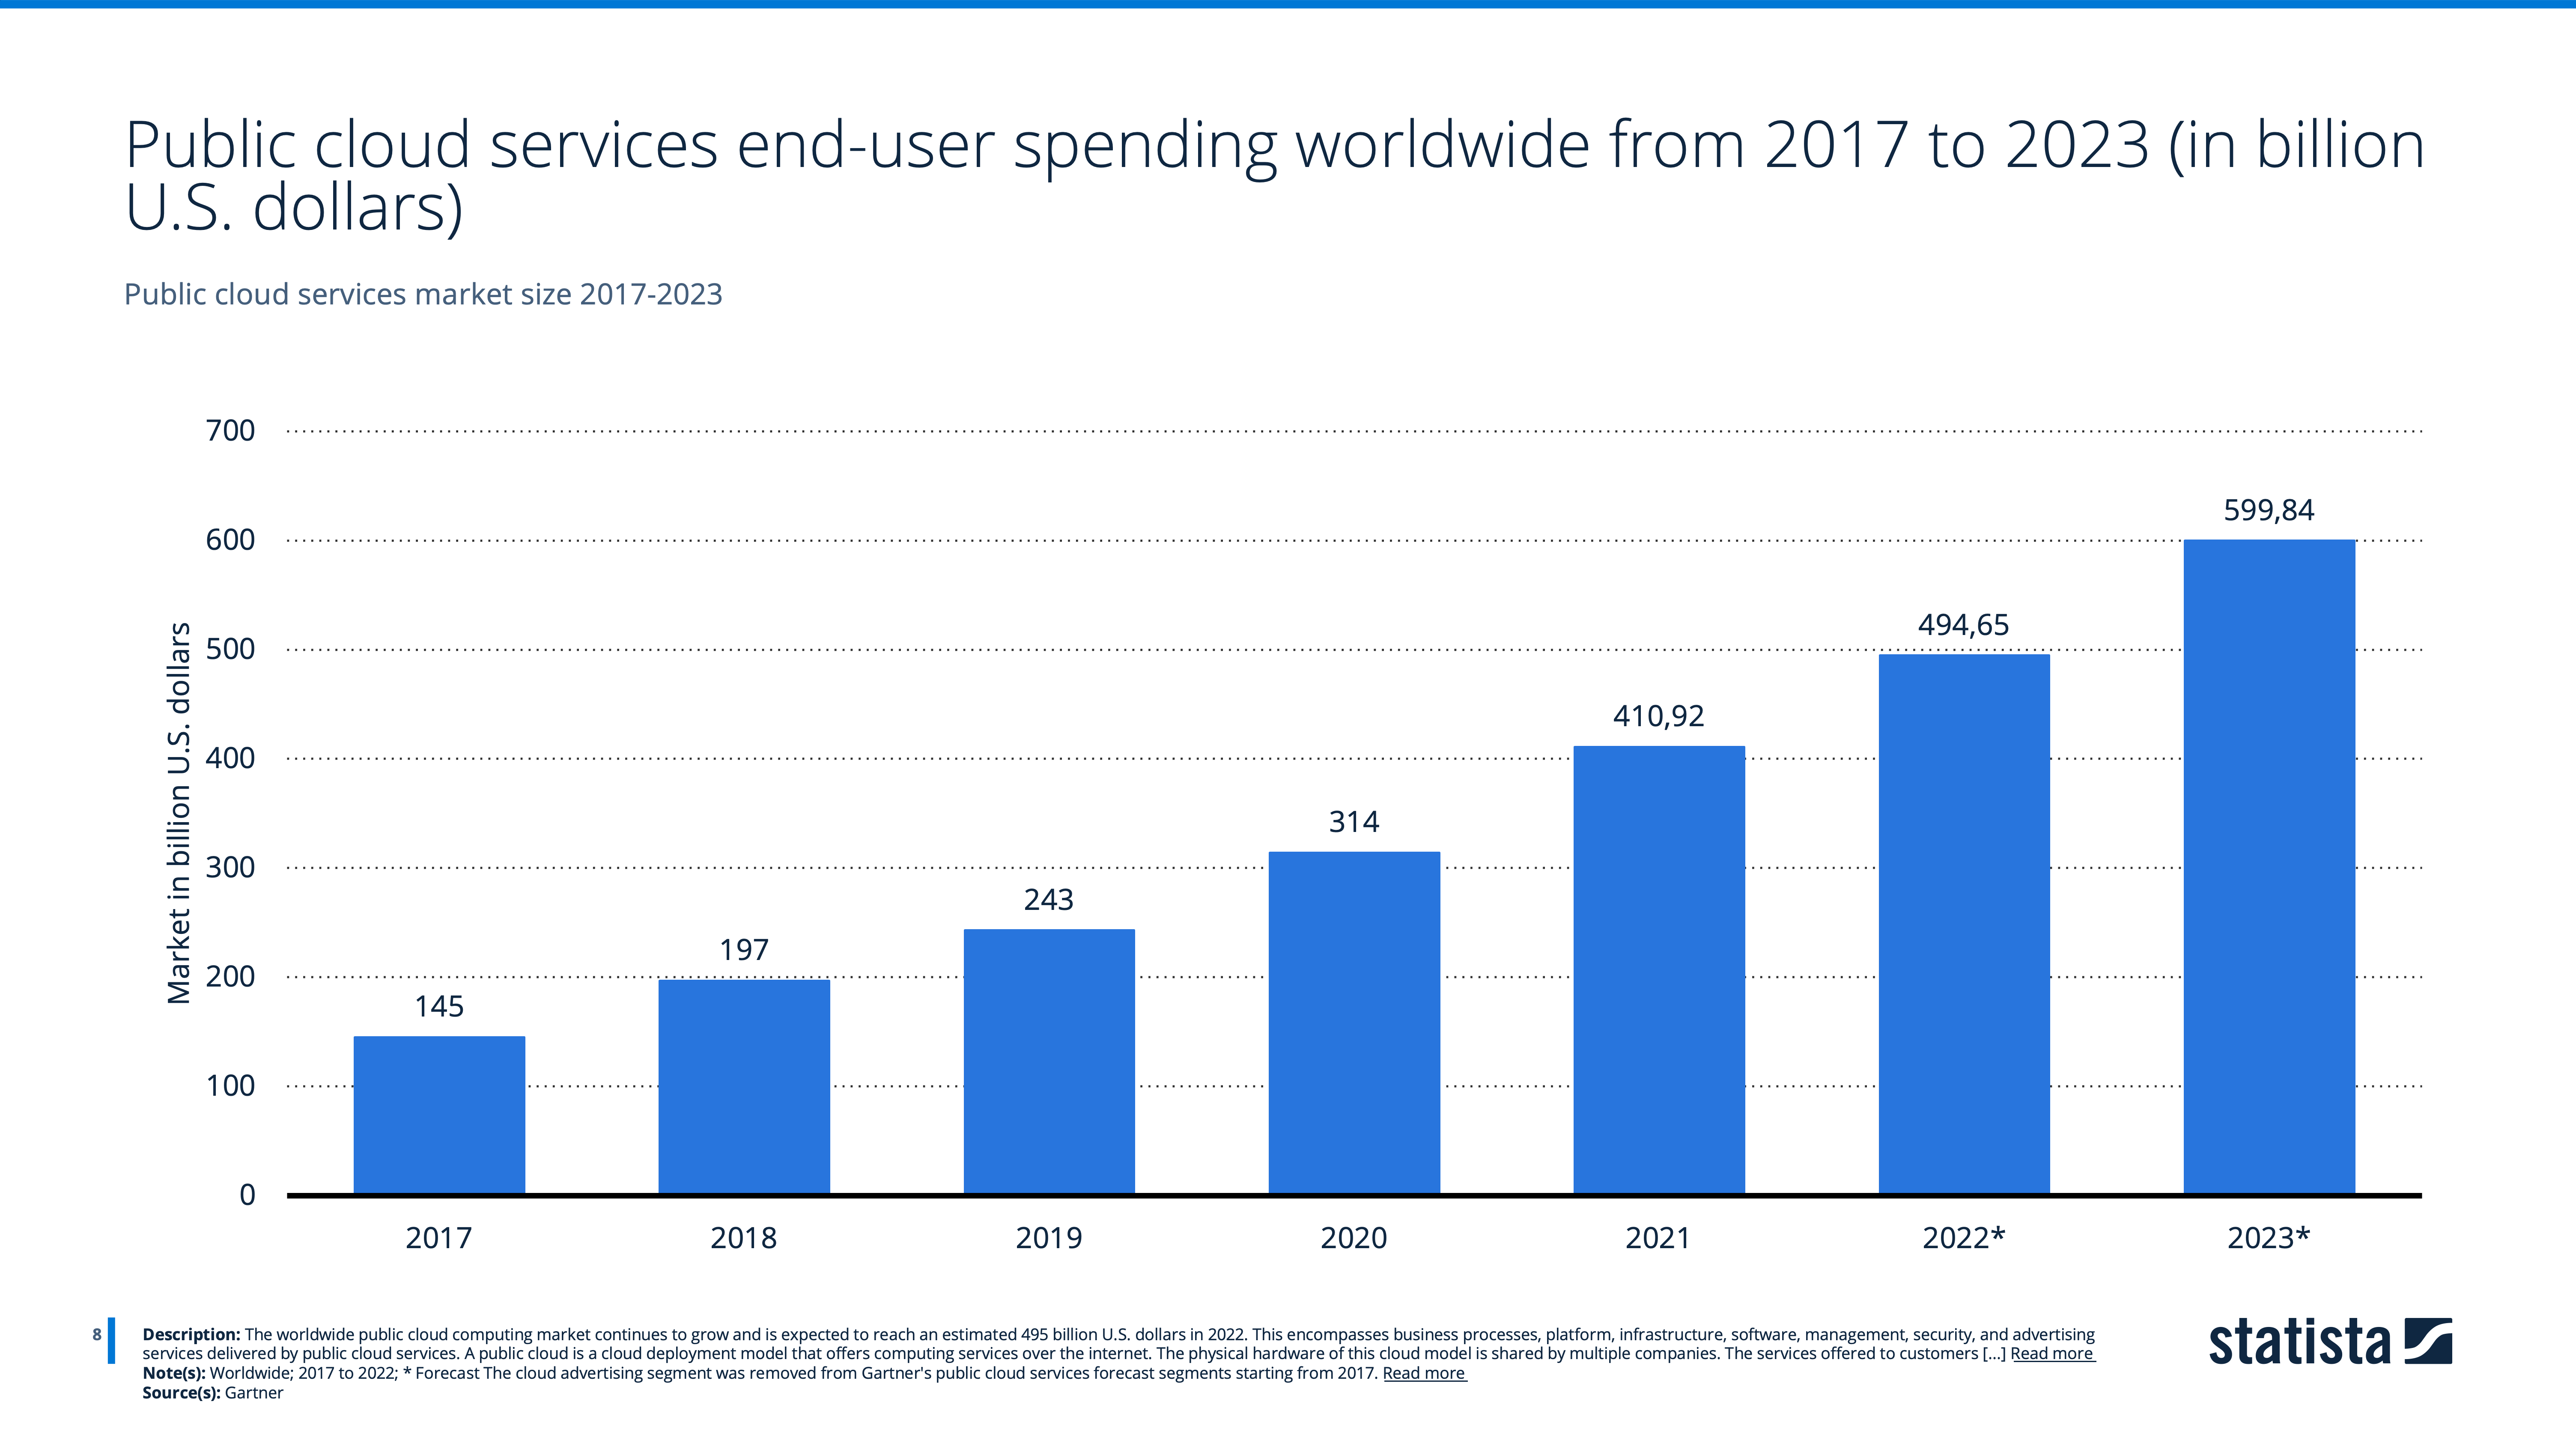
\includegraphics[width=\textwidth]{public_cloud_spending.png}
    \caption{Die Verkaufsleistungen der Public Cloud in den letzten Jahren \cite[S. 8]{Statista2022}}
    \label{fig:public_cloud_spending}
\end{figure}

Aus einem Dossier von Statista 2022 geht in der in Abbildung \ref{fig:public_cloud_spending} gezeigten Statistik hervor, dass sich die Ausgaben für public Cloud Services von 2017 bis 2023 etwas mehr als vervierfacht haben werden \cite[Vgl.][S. 8]{Statista2022}. Auch weitere Statistiken desselben Dossiers machen einen stetig steigenden Trend hinsichtlich des Cloud Computing deutlich \cite[Vgl. unter anderem][S. 11ff]{Statista2022}. 

\pagebreak

\subsection{Herausforderungen -> Migration von Legacy Anwendungen}

Neben der steigenden Nutzung von Cloud Computing und der Entwicklung Cloud basierter Anwendungen können auch legacy Anwendungen von Cloud Computing profitieren, woraus sich der trend abzeichnet, dass auch solche Anwendungen auf eine Cloud Infrastruktur migriert werden um die Ressourcen dieser nutzen zu können und Kosten zu sparen \cite[Vgl.][S. 31]{Maenhaut2016}.
\pagebreak
\section{Migrationsansätze}

Im folgenden Kapitel wird auf die unterschiedlichen Migrationsmethoden des Cloud Computing eingegangen.
Durch die unterschiedlichen Servicelevel bedingt gibt es verschiedene Ansätze, wie die Cloud Migration realisierbar ist \cite[Vgl.][S. 226]{Surianarayanan2019},
angefangen mit dem sogenannten \glqq{Lift and Shift}\grqq{}, bis hin zur Entwicklung Cloud nativer Anwendungen \cite[Vgl.][S. 144]{Zhao2014}.

\subsection{Migration zu IaaS (Replatforming/Rehosting)}
Nach Zhao (2014) ist das Replatforming oder Rehosting die vorgeschlagene Strategie für die Migration zu IaaS \cite[Vgl.][S. 144]{Zhao2014}.
Umgangssprachlich wird diese Vorgehensweise auch als \glqq{Lift and Shift}\grqq{} bezeichnet \cite[Vgl.][]{NetApp}.
Bei diesen Strategien werden Anwendungen lediglich auf einer anderen Hardwareplattform installiert, die Anwendungsarchitektur bleibt dabei
unverändert. Dieser Ansatz bietet eine schnelle Lösung zur Migration \cite[Vgl.][]{CIO}.

Der wahrscheinlich größte Vorteil der Migration zu IaaS ist, dass die Anwendungsarchitektur nicht verändert werden muss und die Migration somit
schnell und ohne großen Aufwand vollzogen werden kann. Ein Nachteil ist dagegen, dass die Migration zu IaaS nicht die vollen Möglichkeiten der
Cloud ausnutzt.

\subsection{Migration zu PaaS (Refactoring/Rebuilding)}
Das Refactoring oder Rebuilding von Anwendungen gehört nach Zhao (2014) zu den empfohlenen Strategien für die Migration zu PaaS \cite[Vgl.][S. 144]{Zhao2014}.
Rebuilding bedeutet, den bisherigen Code zu re-architekten um die Vorteile der Cloud Plattform nutzen zu können \cite[Vgl.][]{CIO}.

\subsection{Migration zu SaaS (Cloud Native Entwicklung)}
Der Schritt zu SaaS ist nach Zhao (2014) auf verschiedenen Wegen zu erreichen. Demnach sei eine Anwendung durch einen SaaS Service entweder zu ersetzen,
enstprechend der SaaS Prinzipien zu überarbeiten oder zu einem SaaS Service unzustrukturieren \cite[Vgl.][S. 144]{Zhao2014}.

Das Augeben einer Anwendung und vollständige Ersetzen dieser durch Nutzung des SaaS Modells bedarf eines
größeren Aufwand und ein Entwicklungsteam zur Umsetzung der Anforderungen \cite[Vgl.][]{CIO}.

Sind die Ressourcen vorhanden, ist die Cloud Native Entwicklung von Anwendungen mit Serverless Functions, auch als
Lambda Funtionen bekannt, möglich.

%title wird unter dem Bsp. abgedruckt
%caption wird im Verzeichnis abgedruckt
%label wird zum referenzieren benutzt, muss einzigartig sein.

% \begin{lstlisting}[caption=Code-Beispiel, label=Bsp.1]
% public class HelloWorld {
% 	public static void main (String[] args) {
% 		// Ausgabe Hello World!
% 		System.out.println("Hello World!");
% 	}
% }
% \end{lstlisting}

% %language ändert die Sprache. (Wenn nur eine Sprache verwendet wird, kann diese Sprache in einstellungen.tex geändert werden. Standardmäßig Java.)
% \begin{lstlisting}[caption=Python-Code, label=Python-Code, title=Titel des Python-Codes,language=Python]
% def quicksort(liste):
% if len(liste) <= 1:
% 	return liste
% pivotelement = liste.pop()
% links = [element for element in liste if element < pivotelement]
% rechts = [element for element in liste if element >= pivotelement]
% return quicksort(links) + [pivotelement] + quicksort(rechts)
% # Quelle: http://de.wikipedia.org/wiki/Python_(Programmiersprache)
% \end{lstlisting}

% \section{Verweis auf Code}
% Verweis auf den Code \autoref{Bsp.1}.\\
% und der Python-Code \autoref{Python-Code}.

% Zweite Erwähnung einer Abkürzung \ac{AGPL} (Erlärung wird nicht mehr angezeigt)